\documentclass[10pt]{article}
\usepackage[a4paper, tmargin=0.75in, lmargin=0.80in, rmargin=0.80in, bmargin=1in]{geometry}
\usepackage{hyperref}
\usepackage{booktabs}
\usepackage{siunitx}
\usepackage{graphicx}
\usepackage{natbib}
\usepackage{tikz}
\usepackage{float}
\usepackage{xcolor}
\usetikzlibrary{automata, positioning, calc}
\usepackage{verbatim}
\usepackage{listings}
\usepackage{amsmath}
\pagestyle{empty}
% In preamble:
\usepackage{tabularx}
\usepackage{booktabs}

%%%%%%%%%%%%%%%%%%%%%%%%%%%%%%%%%%%%%%%%%%%%%%%%%%
% INFORMATION MACROS
%%%%%%%%%%%%%%%%%%%%%%%%%%%%%%%%%%%%%%%%%%%%%%%%%%
\newcommand{\studentname}{Shu-Lin Shih and Jaideep Khare}
\newcommand{\studentnumber}{35199856 and 35193853}
\newcommand{\coursename}{ECE 622: Modeling \& Verification of Embedded Systems}
\newcommand{\semester}{Spring 2026}

%%%%%%%%%%%%%%%%%%%%%%%%%%%%%%%%%%%%%%%%%%%%%%%%%%

\begin{document}

\begin{center}
{\huge{\coursename}} \\
\vspace{2mm}
{\Large{\semester: Lab 1: Reachability Analysis Report}}

% \vspace{2mm}
% {\Large{Reachability Analysis}} \\
\vspace{1mm}
{\Large{Prof. Daniel Holcomb}}
\end{center}

\vspace{5mm}
\hrule
\vspace{1mm}
\hrule

\vspace{3mm}
\begin{tabular}{ll}
Submitted by:  & {\studentname} \\
Student ID:     & {\studentnumber} \\
Lab No.:        & 1 \\
Submission Date:& March 04, 2026 \\
\end{tabular}

\vspace{3mm}
\hrule
\vspace{1mm}
\hrule

%%%%%%%%%%%%%%%%%%%%%%%%%%%%%%%%%%%%%%%%%%%%%%%%%%
\section*{Overview}

This lab explores explicit and symbolic reachability analysis for sequential systems. 
All experiments were performed on Ubuntu 16.04 using MiniSAT and PicoSAT.

Part A uses graph traversal and simulation-based reachability, while Part B implements SAT-based symbolic reachability through CNF encoding and transition relation unrolling. Part C extends the symbolic approach to counting reachable states.


\section{Part A: Reachability by Graph Traversal}

\subsection*{A.1: State Transition Graphs}

For each design, we constructed the state transition graph by enumerating all states and evaluating the next-state for every possible input combination. The transitions were determined either directly from the gate-level schematic (ex1) and applying test vectors using simulation on the hdl file (stoplight1).

\subsubsection*{ex1 Design}

The design \texttt{ex1.v} contains two state bits $(S_1,S_0)$ and one input $A$. Therefore the system has $2^2 = 4$ possible states and $2 \times 4 = 8$ possible $(A,S_1,S_0)$ combinations.

Using the gate-level schematic of \texttt{ex1.v}, we evaluated the next-state logic $(NS_1,NS_0)$ for each combination. The resulting transition truth table is shown in Table~1.

\begin{table}[h]
\centering
\begin{tabular}{c c c | c c}
\toprule
A & S1 & S0 & NS1 & NS0 \\
\midrule
0 & 0 & 0 & 0 & 1 \\
1 & 0 & 0 & 0 & 1 \\
0 & 0 & 1 & 0 & 1 \\
1 & 0 & 1 & 0 & 1 \\
0 & 1 & 0 & 0 & 1 \\
1 & 1 & 0 & 0 & 1 \\
0 & 1 & 1 & 0 & 0 \\
1 & 1 & 1 & 1 & 0 \\
\bottomrule
\end{tabular}
\caption{State transition truth table for \texttt{ex1.v}}
\end{table}

From Table~1, rows that lead to identical state transitions were grouped together and represented as labeled edges in the state transition graph. The resulting FSM is shown in Fig.~1. The initial state is $00$.

\begin{figure}[H]
\centering
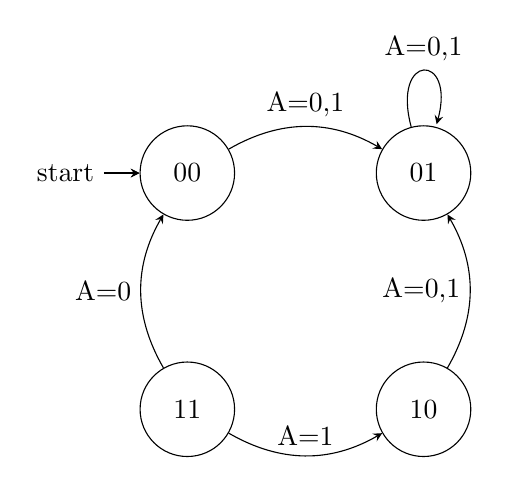
\begin{tikzpicture}[
    ->,
    >=stealth,
    node distance=3cm,
    on grid,
    auto,
    every state/.style={draw, circle, minimum size=1.2cm}
]

% States
\node[state, initial] (S0) {$00$};
\node[state] (S1) [right=of S0] {$01$};
\node[state] (S3) [below=of S0] {$11$};
\node[state] (S2) [right=of S3] {$10$};

% Initial arrow
\draw[->] ($(S0)+(-1.0,0)$) -- (S0);

% Transitions
\path
(S0) edge[bend left] node {A=0,1} (S1)
(S1) edge[loop above] node {A=0,1} (S1)
(S2) edge[bend right] node {A=0,1} (S1)
(S3) edge[bend right] node {A=1} (S2)
(S3) edge[bend left] node[left] {A=0} (S0);

\end{tikzpicture}
\caption{State transition graph for \texttt{ex1.v}, only \{0,1\} is reachable from initial}
\end{figure}

\subsubsection*{stoplight1 Design}

The design \texttt{stoplight1.v} contains four state bits, resulting in $2^4 = 16$ possible states. For each state $S \in \{0000,0001,\dots,1111\}$ we evaluated the next state for both values of the pedestrian input signal (\texttt{Ped}=0 and \texttt{Ped}=1) by simulating the design in AMD Vivado HDL Simulator screenshot as shown. 

Using the transition relations obtained from simulation results (Fig. 2), we constructed the FSM shown in Fig.~3. Each node represents a 4-bit state and each directed edge is labeled with the corresponding input value of \texttt{Ped}.

% \textbf{Simulation screenshots (placeholders):}
\begin{figure}[H]
\centering
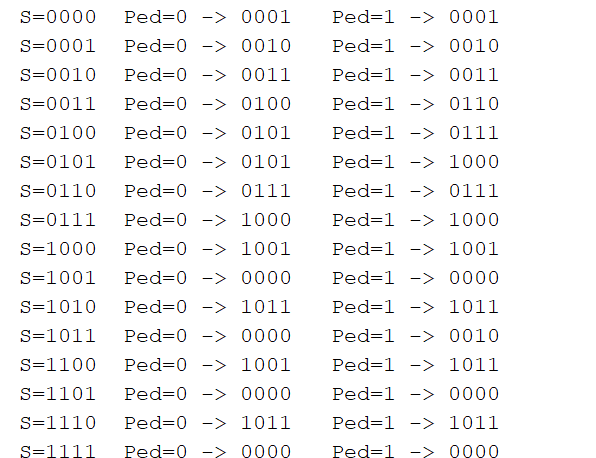
\includegraphics[width=0.60\textwidth]{A1stoplight1sim.png}
\caption{Screenshot for \texttt{stoplight1.v} testbench simulation}
\label{fig:a4_ex1}
\end{figure}
%----------------------------------------------------------------------------------------------------
\begin{figure}[H]
% \centering
\raggedright
\hspace{2.5cm}
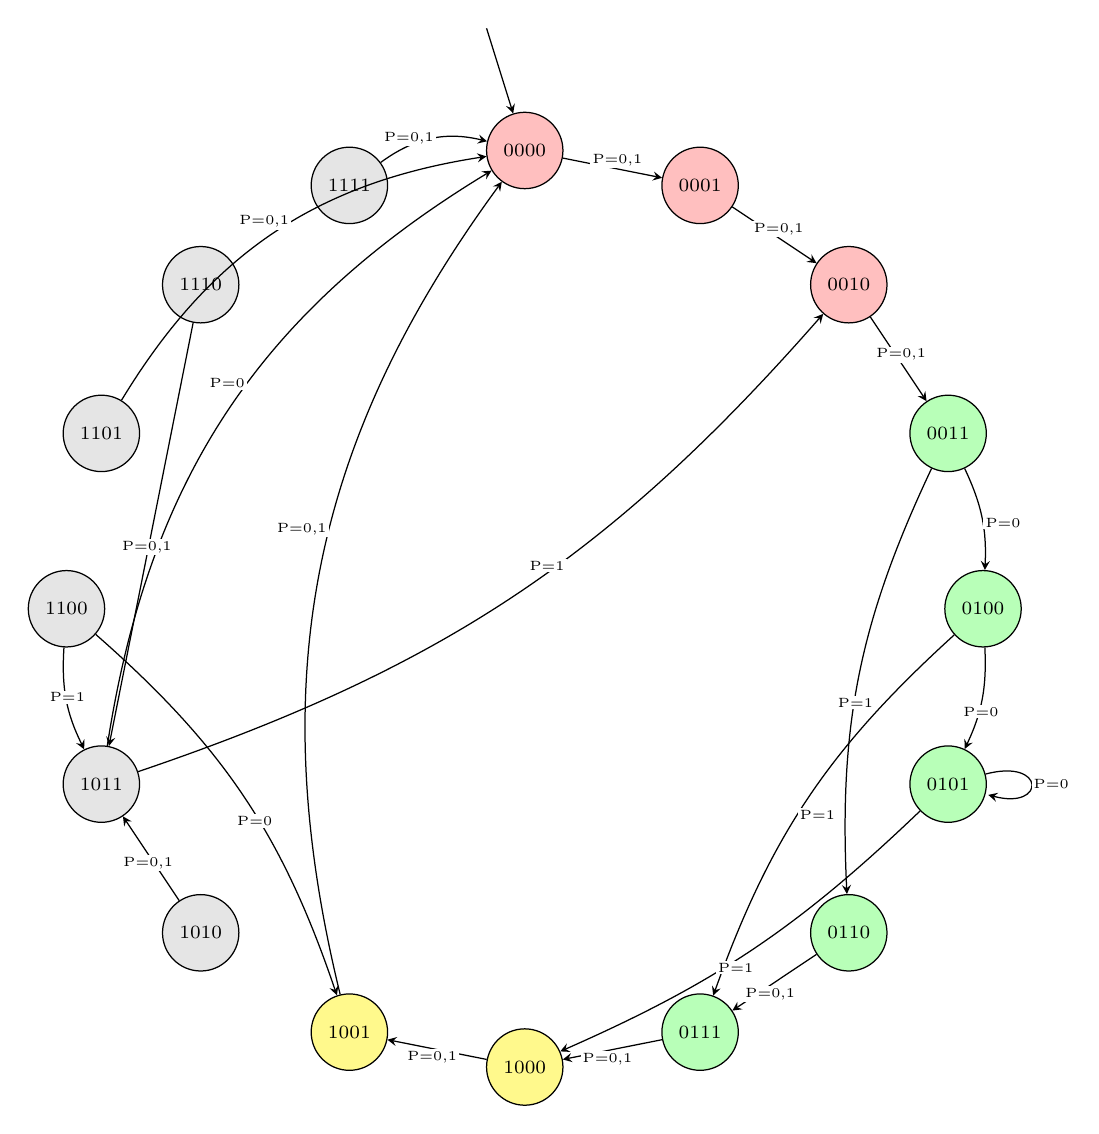
\begin{tikzpicture}[
    ->,
    >=stealth,
    scale=0.97,                 % GLOBAL scaling of entire figure
    transform shape,
    every state/.style={draw, circle, minimum size=10mm, font=\scriptsize},
    edgelab/.style={font=\tiny, fill=white, inner sep=0.8pt},
    line width=0.45pt,
    greenstate/.style={fill=green!28},
    yellowstate/.style={fill=yellow!45},
    redstate/.style={fill=red!25},
    invalidstate/.style={fill=gray!20},
]

% -------------------------------------------------
% Background sector shading (paper-style grouping)
% -------------------------------------------------
% circle radius used for node placement is 6, so shade slightly larger
% \begin{scope}[on background layer]
%     % EW Green sector (around 45° to 22.5° nodes: 0010,0011)
%     \fill[green!10] (0,0) -- (45:6.9) arc (45:10:6.9) -- cycle;

%     % EW Yellow sector (near 67.5° node: 0001)
%     \fill[yellow!12] (0,0) -- (80:6.9) arc (80:55:6.9) -- cycle;

%     % NS Green sector (bottom-left around -90° to -112.5° nodes: 1000,1001)
%     \fill[green!10] (0,0) -- (-75:6.9) arc (-75:-130:6.9) -- cycle;

%     % NS Yellow sector (right side around 0° to -22.5° nodes: 0100,0101)
%     \fill[yellow!12] (0,0) -- (10:6.9) arc (10:-35:6.9) -- cycle;

%     % All-red / other sector (remaining states)
%     \fill[red!8] (0,0) -- (180:6.9) arc (180:80:6.9) -- cycle;
%     \fill[red!8] (0,0) -- (55:6.9) arc (55:10:6.9) -- cycle;
%     \fill[red!8] (0,0) -- (-35:6.9) arc (-35:-75:6.9) -- cycle;
%     \fill[red!8] (0,0) -- (-130:6.9) arc (-130:-180:6.9) -- cycle;
% \end{scope}

% -------------------------------------------------
% Nodes (colored by semantic meaning)
% Assumption consistent with typical stoplight encoding used in labs:
% bits correspond to which lamp is active -> map to red/yellow/green phase.
% -------------------------------------------------

% --- Circular layout (colored by SigG/SigY/SigR from stoplight1.v) ---
\node[state,redstate]    (s0000) at (90:6) {0000};
\node[state,redstate]    (s0001) at (67.5:6) {0001};
\node[state,redstate]    (s0010) at (45:6) {0010};
\node[state,greenstate]  (s0011) at (22.5:6) {0011};

\node[state,greenstate]  (s0100) at (0:6) {0100};
\node[state,greenstate]  (s0101) at (-22.5:6) {0101};
\node[state,greenstate]  (s0110) at (-45:6) {0110};
\node[state,greenstate]  (s0111) at (-67.5:6) {0111};

\node[state,yellowstate] (s1000) at (-90:6) {1000};
\node[state,yellowstate] (s1001) at (-112.5:6) {1001};

\node[state,invalidstate] (s1010) at (-135:6) {1010};
\node[state,invalidstate] (s1011) at (-157.5:6) {1011};

\node[state,invalidstate] (s1100) at (180:6) {1100};
\node[state,invalidstate] (s1101) at (157.5:6) {1101};
\node[state,invalidstate] (s1110) at (135:6) {1110};
\node[state,invalidstate] (s1111) at (112.5:6) {1111};

% Initial arrow (into 0000)
\draw[->] ($(s0000)+(-0.5,1.6)$) -- (s0000);

% -------------------------------------------------
% Transitions (labels small + boxed)
% -------------------------------------------------
\path
(s0000) edge node[pos=0.55, edgelab, above] {P=0,1} (s0001)
(s0001) edge node[pos=0.55, edgelab, above] {P=0,1} (s0010)
(s0010) edge node[pos=0.55, edgelab, above] {P=0,1} (s0011)

(s0011) edge[bend left=14]  node[pos=0.55, edgelab, right] {P=0} (s0100)
(s0011) edge[bend right=14] node[pos=0.55, edgelab, below] {P=1} (s0110)

(s0100) edge[bend left=14]  node[pos=0.55, edgelab, below] {P=0} (s0101)
(s0100) edge[bend right=14] node[pos=0.55, edgelab, right] {P=1} (s0111)

(s0101) edge[loop right] node[edgelab] {P=0} (s0101)
(s0101) edge[bend left=10] node[pos=0.55, edgelab, below] {P=1} (s1000)

(s0110) edge node[pos=0.55, edgelab, below] {P=0,1} (s0111)
(s0111) edge node[pos=0.55, edgelab, below] {P=0,1} (s1000)

(s1000) edge node[pos=0.55, edgelab, below] {P=0,1} (s1001)
(s1001) edge[bend left=25] node[pos=0.55, edgelab, left] {P=0,1} (s0000)

(s1010) edge node[pos=0.55, edgelab, below] {P=0,1} (s1011)

(s1011) edge[bend left=25]  node[pos=0.55, edgelab, left] {P=0} (s0000)
(s1011) edge[bend right=15] node[pos=0.55, edgelab, above] {P=1} (s0010)

(s1100) edge[bend left=15]  node[pos=0.55, edgelab, below] {P=0} (s1001)
(s1100) edge[bend right=15] node[pos=0.55, edgelab, above] {P=1} (s1011)

(s1101) edge[bend left=25] node[pos=0.55, edgelab, left] {P=0,1} (s0000)
(s1110) edge node[pos=0.55, edgelab, above] {P=0,1} (s1011)
(s1111) edge[bend left=25] node[pos=0.55, edgelab, left] {P=0,1} (s0000);


% -------------------------------------------------
% % Legend
% \begin{scope}[shift={(0,-9.0)}]
%   \node[draw,circle,fill=green!28,minimum size=5mm] at (-3,0) {};
%   \node[font=\scriptsize] at (-1.9,0) {SigG=1};

%   \node[draw,circle,fill=yellow!45,minimum size=5mm] at (0.7,0) {};
%   \node[font=\scriptsize] at (2.1,0) {SigY=1};

%   \node[draw,circle,fill=red!25,minimum size=5mm] at (4.4,0) {};
%   \node[font=\scriptsize] at (5.8,0) {SigR=1};

%   \node[draw,circle,fill=gray!20,minimum size=5mm] at (8.0,0) {};
%   \node[font=\scriptsize] at (9.7,0) {unreachable};
% \end{scope}

\end{tikzpicture}
\center
\caption{Complete state transition graph for \texttt{stoplight1.v}. States are color-coded for readability. Unreachability is indicated using grey-colored state circles with respect to given initial state 0000.}
\end{figure}



% ============================
% Part A (A.2, A.3, A.4, A.5)
% ============================

\subsection*{A.2: Target Reachability and Shortest Path}

\textbf{ex1: target state 11 is unreachable.}
From the state transition graph of \texttt{ex1.v}, the initial state is $00$ and it transitions to $01$ for both $A=0$ and $A=1$.
State $01$ then self-loops for both $A=0$ and $A=1$, so the machine becomes trapped in $01$ after at most one transition.
Therefore, state $11$ is not reachable from the initial state $00$ under any input sequence.

\vspace{2mm}

\noindent
\textbf{stoplight1: shortest path to target state 0100.}
From the state transition graph of \texttt{stoplight1.v}, the following shortest path (4 transitions) reaches the target state $0100$ from the initial state $0000$:
% \[
% 0000 \xrightarrow{\texttt{Ped}=0/1} 0001 \xrightarrow{\texttt{Ped}=0/1} 0010 \xrightarrow{\texttt{Ped}=0/1} 0011 \xrightarrow{\texttt{Ped}=0} 0100
% \]


% ------------------------------------------------------------
% stoplight1 full FSM (circular) with red-highlighted shortest path
% ------------------------------------------------------------
\begin{figure}[H]
\centering
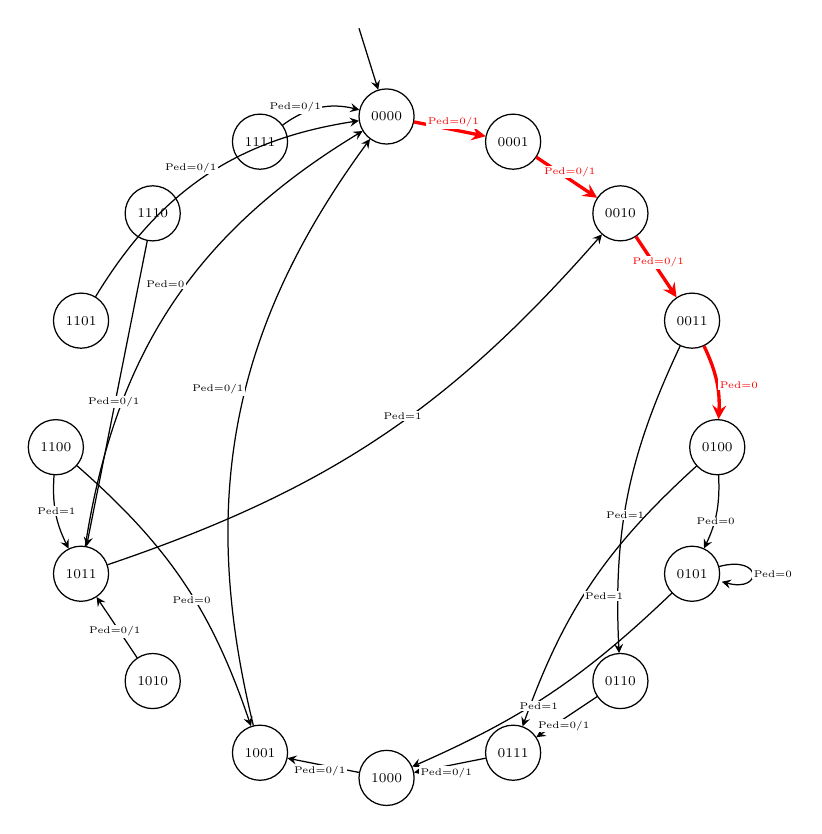
\begin{tikzpicture}[
    ->,
    >=stealth,
    scale=0.70,
    transform shape,
    every state/.style={draw, circle, minimum size=10mm, font=\scriptsize},
    edgelab/.style={font=\tiny, fill=white, inner sep=0.8pt},
    line width=0.45pt
]

% --- Circular layout ---
\node[state] (s0000) at (90:6) {0000};
\node[state] (s0001) at (67.5:6) {0001};
\node[state] (s0010) at (45:6) {0010};
\node[state] (s0011) at (22.5:6) {0011};

\node[state] (s0100) at (0:6) {0100};
\node[state] (s0101) at (-22.5:6) {0101};
\node[state] (s0110) at (-45:6) {0110};
\node[state] (s0111) at (-67.5:6) {0111};

\node[state] (s1000) at (-90:6) {1000};
\node[state] (s1001) at (-112.5:6) {1001};
\node[state] (s1010) at (-135:6) {1010};
\node[state] (s1011) at (-157.5:6) {1011};

\node[state] (s1100) at (180:6) {1100};
\node[state] (s1101) at (157.5:6) {1101};
\node[state] (s1110) at (135:6) {1110};
\node[state] (s1111) at (112.5:6) {1111};

% Initial arrow (into 0000)
\draw[->] ($(s0000)+(-0.5,1.6)$) -- (s0000);

% --- Transitions ---
% Highlight shortest path edges in RED + thicker
\path
(s0000) edge[red, very thick] node[pos=0.55, edgelab, above] {Ped=0/1} (s0001)
(s0001) edge[red, very thick] node[pos=0.55, edgelab, above] {Ped=0/1} (s0010)
(s0010) edge[red, very thick] node[pos=0.55, edgelab, above] {Ped=0/1} (s0011)

% Final step of shortest path requires Ped=0
(s0011) edge[red, very thick, bend left=14] node[pos=0.55, edgelab, right] {Ped=0} (s0100)

% Remaining edges (normal style)
(s0011) edge[bend right=14] node[pos=0.55, edgelab, below] {Ped=1} (s0110)

(s0100) edge[bend left=14]  node[pos=0.55, edgelab, below] {Ped=0} (s0101)
(s0100) edge[bend right=14] node[pos=0.55, edgelab, right] {Ped=1} (s0111)

(s0101) edge[loop right] node[edgelab] {Ped=0} (s0101)
(s0101) edge[bend left=10] node[pos=0.55, edgelab, below] {Ped=1} (s1000)

(s0110) edge node[pos=0.55, edgelab, below] {Ped=0/1} (s0111)
(s0111) edge node[pos=0.55, edgelab, below] {Ped=0/1} (s1000)

(s1000) edge node[pos=0.55, edgelab, below] {Ped=0/1} (s1001)
(s1001) edge[bend left=25] node[pos=0.55, edgelab, left] {Ped=0/1} (s0000)

(s1010) edge node[pos=0.55, edgelab, below] {Ped=0/1} (s1011)

(s1011) edge[bend left=25]  node[pos=0.55, edgelab, left] {Ped=0} (s0000)
(s1011) edge[bend right=15] node[pos=0.55, edgelab, above] {Ped=1} (s0010)

(s1100) edge[bend left=15]  node[pos=0.55, edgelab, below] {Ped=0} (s1001)
(s1100) edge[bend right=15] node[pos=0.55, edgelab, above] {Ped=1} (s1011)

(s1101) edge[bend left=25] node[pos=0.55, edgelab, left] {Ped=0/1} (s0000)
(s1110) edge node[pos=0.55, edgelab, above] {Ped=0/1} (s1011)
(s1111) edge[bend left=25] node[pos=0.55, edgelab, left] {Ped=0/1} (s0000);

\end{tikzpicture}
\caption{State transition graph for \texttt{stoplight1.v}. The shortest path from $0000$ to target $0100$ is highlighted in red.}
\label{fig:stoplight1_path}
\end{figure}

% ------------------------------------------------------------
% A.3
% ------------------------------------------------------------
\subsection*{A.3: States Reachable Within 20 transitions}

For \texttt{ex1.v}, the reachable set saturates immediately: from initial $00$, the machine reaches $01$ in one step and then self-loops forever, so the number of reachable states within $i$ transitions is constantly 2 for $i \ge 1$.

\begin{table}[H]
\centering
\begin{tabular}{c|c}
\toprule
$i \in \{1,2,\dots,20\}$ & \# Reachable states within $i$ transitions (ex1) \\
\midrule
1  & 1 (not counting initial state) \\
2  & 1 \\
3  & 1 \\
4  & 1 \\
5  & 1 \\
6  & 1 \\
7  & 1 \\
8  & 1 \\
9  & 1 \\
10 & 1 \\
11 & 1 \\
12 & 1 \\
13 & 1 \\
14 & 1 \\
15 & 1 \\
16 & 1 \\
17 & 1 \\
18 & 1 \\
19 & 1 \\
20 & 1 \\
\bottomrule
\end{tabular}
\caption{Cumulative reachable-state counts for \texttt{ex1.v}, from the initial state \{00\}.}
\label{tab:a3_ex1}
\end{table}


For \texttt{stoplight1.v}, the number of reachable states grows over the first few transitions and then saturates at 10 states.
The increase in reachable states from 3 to 5 (when $j$ increases from $3$ to $4$) occurs because different values of \texttt{Ped} introduce branching transitions that can shorten the green-light phase. This branching allows the system to reach additional states that are not accessible under a single deterministic input sequence. Overall, the design contains a total of ten valid states: three Red states, five Green states, and two Yellow states. All of these states become reachable once the exploration depth satisfies $i \ge 8$, after which the reachable set saturates and no new states are discovered.


\begin{table}[h]
\centering
\begin{tabular}{c|c}
\toprule
$i \in \{1,2,\dots,20\}$ & \# Reachable states within $i$ transitions (stoplight1) \\
\midrule
1  & 1 \\
2  & 2 \\
3  & 3 \\
4  & 5 \\
5  & 7 \\
6  & 8 \\
7  & 9 \\
8  & 10 \\
9  & 10 \\
10 & 10 \\
11 & 10 \\
12 & 10 \\
13 & 10 \\
14 & 10 \\
15 & 10 \\
16 & 10 \\
17 & 10 \\
18 & 10 \\
19 & 10 \\
20 & 10 \\
\bottomrule
\end{tabular}
\caption{Cumulative reachable-state counts for \texttt{stoplight1.v}, from the initial state \{0000\}.}
\label{tab:a3_stoplight1}
\end{table}
% ------------------------------------------------------------
% A.4
% ------------------------------------------------------------
\subsection*{A.4: Random Execution Using Verilog Testbench}

A Verilog testbench was written to explore reachability using random simulation. The testbench (code snapshot included in appendix) performs the following steps:

\begin{itemize}
\item Forces the initial state of the FSM to the reset state.
\item Applies random input values every clock cycle.
\item Checks at each cycle whether the target state has been reached.
\item Terminates immediately if the target state is reached.
\item Stops the experiment after 100{,}000 cycles if the target state is never observed.
\end{itemize}
\vspace{0.3cm}
\noindent
\textbf{Observed simulation outcomes:}

\begin{itemize}
\item \texttt{ex1}: Target state \texttt{11} was \textbf{not reached} within 100{,}000 cycles (timeout).
\item \texttt{ex2}: Target state \texttt{1111111111111} was \textbf{not reached} within 100{,}000 cycles (timeout).
\item \texttt{stoplight1}: Target state \texttt{0100} was \textbf{reached at cycle 52}.
\item \texttt{stoplight2}: Target state \texttt{01000} was \textbf{reached at cycle 1357}.
\end{itemize}

The simulation logs confirming these results are shown in the figures below.

\begin{figure}[H]
\centering
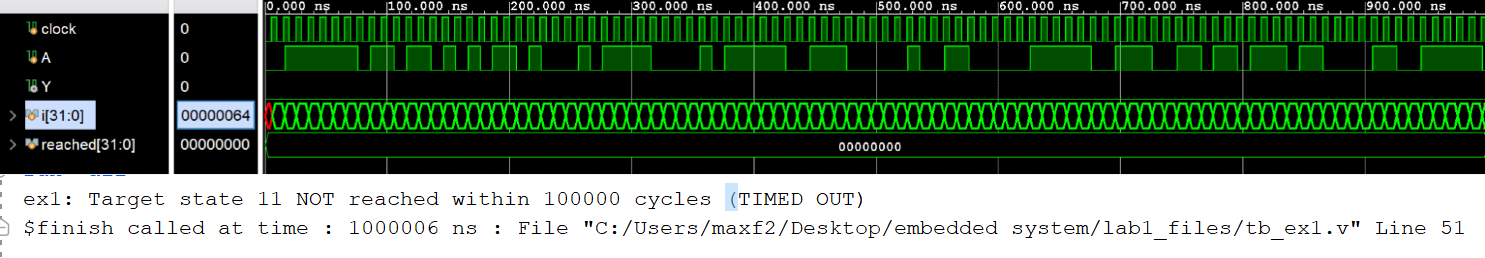
\includegraphics[width=0.9\textwidth]{ex1final.png}
\caption{Waveform for \texttt{ex1}. Target state \texttt{11} was not reached within the simulation limit of 100{,}000 cycles.}
\end{figure}

\begin{figure}[H]
\centering
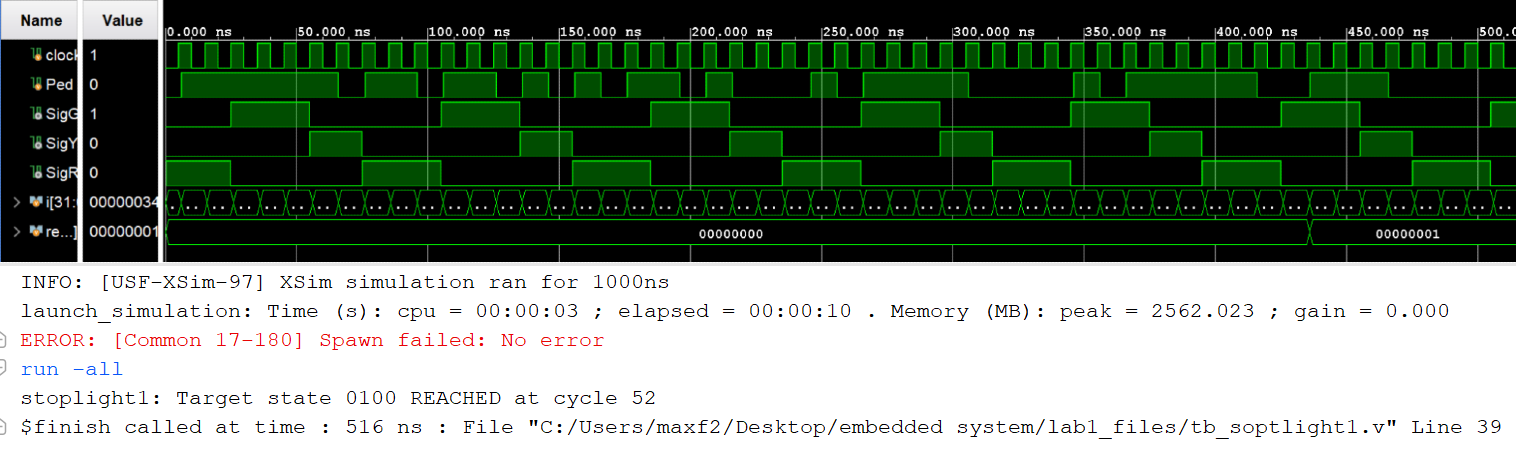
\includegraphics[width=0.9\textwidth]{stoplight1final.png}
\caption{Waveform for \texttt{stoplight1}. Target state \texttt{0100} was reached during random simulation.}
\end{figure}

\begin{figure}[H]
\centering
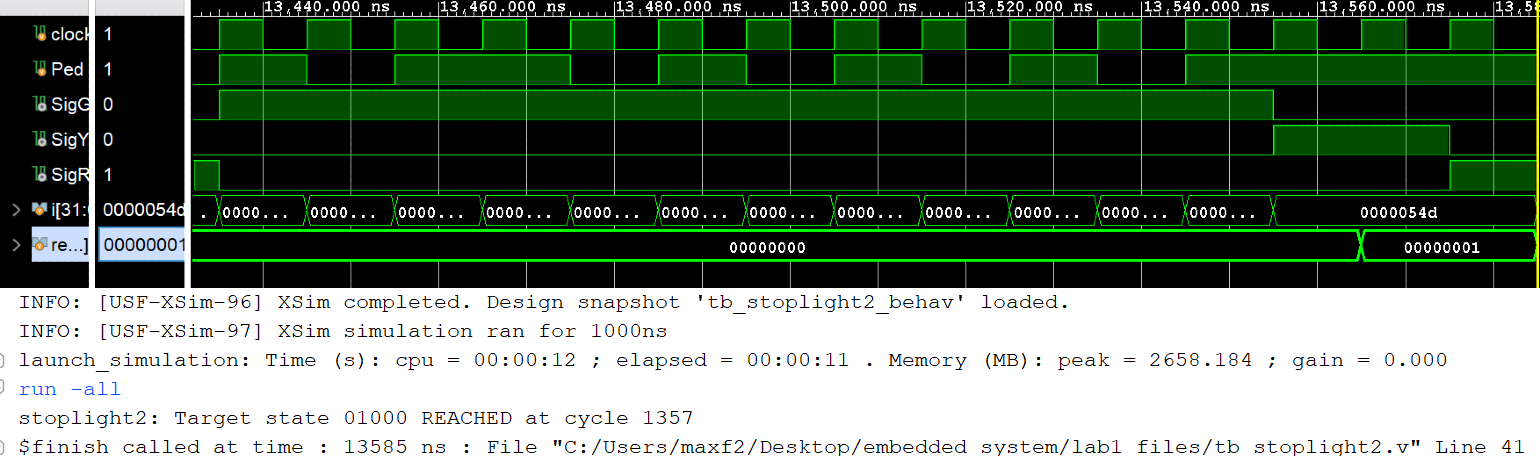
\includegraphics[width=0.9\textwidth]{stoplight2final.png}
\caption{Waveform for \texttt{stoplight2}. Target state \texttt{01000} was reached at cycle 1357.}
\end{figure}

\begin{figure}[H]
\centering
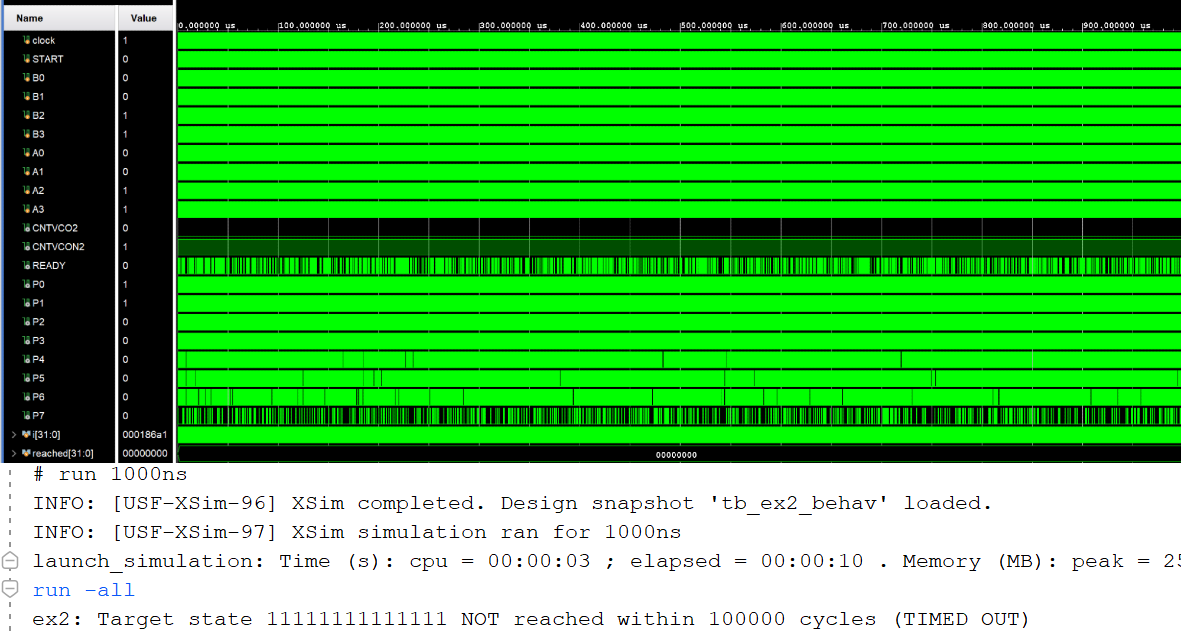
\includegraphics[width=0.9\textwidth]{ex2final.png}
\caption{Waveform for \texttt{ex2}. Target state was not reached during the simulation interval.}
\end{figure}

We conclude that while this approach provides a practical way to observe reachability behavior in simulation, it does not guarantee exploration of all possible input sequences. 
% ------------------------------------------------------------
% A.5
% ------------------------------------------------------------
\subsection*{A.5: Consistency Between Graph Analysis and Simulation}

For \texttt{stoplight1}, the simulation result is found to be consistent with the reachability predicted by the transition graph.

\vspace{0.3cm}
\noindent
\textbf{Analysis on different approaches (A.2 and A.4):}
% \noindent
% From the transition graph analysis in Section A.2, the shortest path from the initial state to the target state \texttt{0100} requires atleast four transitions. However, during random simulation the target state was reached at \textbf{cycle 52}. This difference occurs because the simulation uses randomly generated inputs. The required input sequence that leads to the shortest path may not appear immediately.

% This occurs because we observe the state transition graph contains branches (for example transitions toward state \texttt{0110}), which may divert the machine away from the direct path to the target state. Because the inputs are random, the FSM may follow several alternative transitions before eventually encountering the correct sequence that leads to \texttt{0100}. This explains why the target state appeared later in simulation.
\noindent
From the graph analysis in A.2, the target state \texttt{0100} is reachable from the initial state, and the shortest path requires atleast four transitions. In the random simulation experiment of A.4, the target state was reached at cycle 52. The larger number of cycles occurs because the simulation uses randomly generated inputs. 

The FSM may take alternative branches in the transition graph (for example transitions through state \texttt{0110}) before eventually following the sequence that leads to the target state.

A finding that would indicate an error in the earlier analysis would be if the simulation \emph{never} reached state \texttt{0100} even after a very large number of cycles. Since the transition graph shows that this state is reachable, such a result would imply that either the graph analysis in A.2 or the simulation setup in A.4 was incorrect.

% \vspace{0.3cm}
% \noindent
% \textbf{stoplight2:}
% \noindent
% The target state \texttt{01000} was eventually reached during random simulation (cycle 1357), confirming that the state is reachable from the initial state. The relatively large number of cycles required again reflects the randomness of the input sequence rather than the actual shortest transition distance in the state graph.


% \vspace{0.3cm}
% \noindent
% \textbf{ex1:}
% \noindent
% The graph analysis showed that state \texttt{11} is unreachable from the initial state \texttt{00}. The random simulation result is consistent with this conclusion, since the target state was not observed even after 100{,}000 cycles of execution.


% \vspace{0.3cm}
% \noindent
% \textbf{ex2:}
% \noindent
% Similarly, the target state \texttt{1111111111111} was not reached during simulation. This suggests that the state is either unreachable or extremely unlikely to occur through random input sequences.


\vspace{0.3cm}
\noindent
\textbf{Discussion:}
\noindent
These results illustrate an important limitation of random simulation. While random execution over many cycles can provide evidence about reachability, it cannot formally guarantee that a state is unreachable. For complex circuits, simulation may require extremely long runtimes before a rare input sequence appears.

Therefore, more systematic techniques such as symbolic execution, SAT-based bounded model checking, or formal reachability analysis are required to accurately determine circuit behavior and prove whether a state is reachable or unreachable.


%%%%%%%%%%%%%%%%%%%%%%%%%%%%%%%%%%%%%%%%%%%%%%%%%%
\section{Part B: SAT-Based Symbolic Reachability}

In this part, we implemented symbolic reachability using CNF encoding and SAT solving.

\subsection*{Program Overview}

Our C++ program performs the following steps:

\begin{enumerate}
\item Parse Verilog netlist.
\item Generate Boolean variables for each node.
\item Encode AND and NOT gates into CNF.
\item Unroll transition relation k times.
\item Add initial state constraints.
\item Add target state constraint at transition k.
\item Output DIMACS CNF and node mapping.
\end{enumerate}

% Data structures used:
% \begin{itemize}
% \item Hash map: Node $\rightarrow$ DIMACS variable index.
% \item Vector of clauses for CNF storage.
% \item Transition relation builder function.
% \end{itemize}


% ------------------------------------------------------------
% B.1
% ------------------------------------------------------------
\subsection*{B.1: ex1 Unrolled 2 Times}

Using the SAT-based reachability tool, the FSM in \texttt{ex1.v} was unrolled for $k=2$ transitions starting from the initial state \texttt{00}. Each possible target state was checked independently.

\vspace{0.25cm}
\noindent
\textbf{Target state 11}

The SAT solver returned \textbf{UNSAT}, meaning no assignment of inputs allows the FSM to reach state \texttt{11} within two transitions.

This is consistent with the transition graph derived in Section A.1, where the FSM moves from \texttt{00} to \texttt{01} and remains trapped in the self-loop at \texttt{01}.

\begin{figure}[H]
\centering
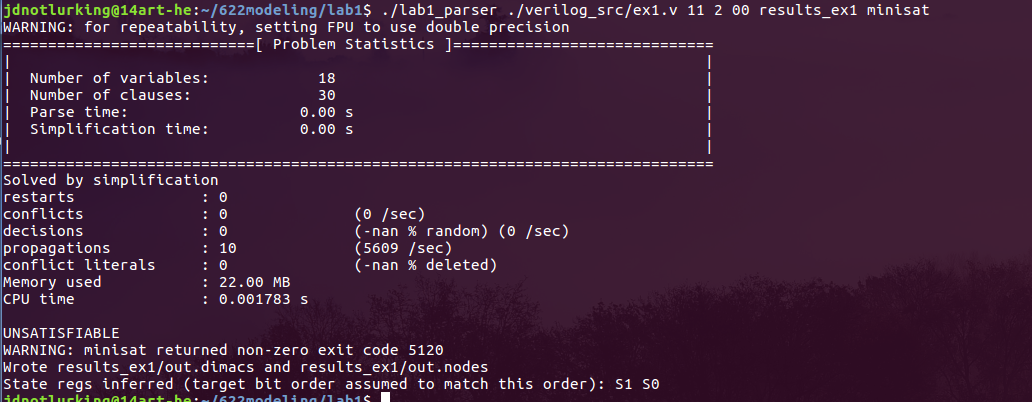
\includegraphics[width=0.9\textwidth]{11ex1.png}
\caption{SAT solver output for target state 11 (UNSAT).}
\end{figure}

\vspace{0.25cm}
\noindent
\textbf{Target state 00}

The solver returned \textbf{UNSAT}. Once the FSM leaves state \texttt{00}, it cannot return to it within the given transition structure.

\begin{figure}[H]
\centering
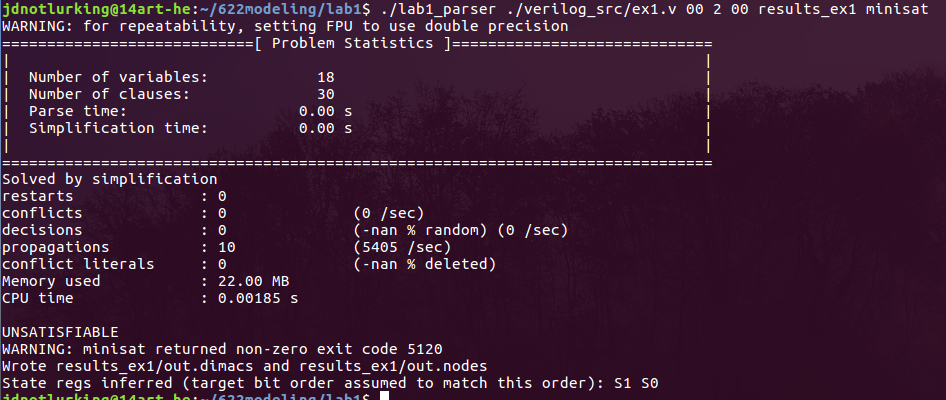
\includegraphics[width=0.9\textwidth]{00ex1.png}
\caption{SAT solver output for target state 00 (UNSAT).}
\end{figure}

\vspace{0.25cm}
\noindent
\textbf{Target state 01}

The solver returned \textbf{SAT}. This state is reachable from the initial state in one transition and contains a self-loop, meaning it remains reachable for any unrolling depth $k \geq 1$.


% \[
% S_1S_0 = 01
% \]

\begin{figure}[H]
\centering
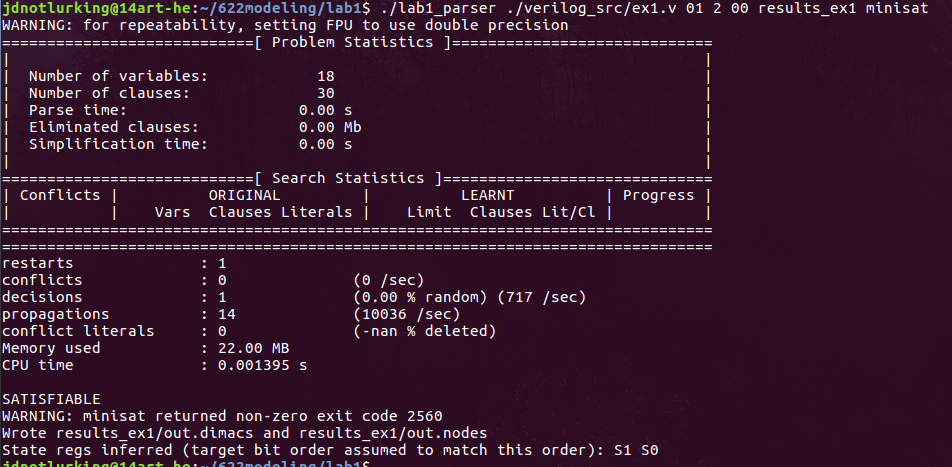
\includegraphics[width=0.9\textwidth]{01ex1.png}
\caption{SAT solver output showing reachability of state 01.}
\end{figure}

\textbf{Target state 10}

The solver returned \textbf{UNSAT}, confirming that state \texttt{10} is not reachable from the initial state \texttt{00} within two transitions.

\begin{figure}[H]
\centering
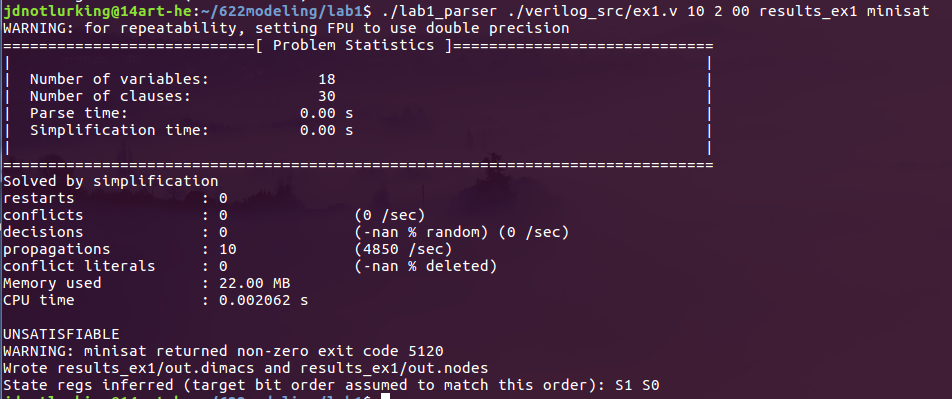
\includegraphics[width=0.9\textwidth]{10ex1.png}
\caption{SAT solver output for target state 10 (UNSAT).}
\end{figure}

% ------------------------------------------------------------
% B.2
% ------------------------------------------------------------
\subsection*{B.2: 15-Step Reachability Analysis}

The transition relation of each design was unrolled for $k=15$ steps and encoded into a CNF formula. The resulting DIMACS file was solved using MiniSAT to determine whether the specified target state is reachable from the initial state.

\begin{table}[H]
\centering
\begin{tabular}{c|c|c}
Design & Reachable within 15 steps? & SAT Result \\
\hline
ex1 & No & UNSAT \\
ex2 & No & UNSAT \\
ex3 & Yes & SAT \\
ex4 & No & UNSAT \\
ex5 & No & UNSAT \\
stoplight1 & Yes & SAT \\
stoplight2 & Yes & SAT \\
\end{tabular}
\caption{Reachability results for 15-step unrolling (same for minisat and picosat)}
\end{table}

\begin{table}[H]
\centering
\begin{tabular}{c|c|c|c|c}
Design & \#Variables & \#Clauses & MiniSAT CPU Time (s) & PicoSAT Time (s) \\
\hline
ex1 & 122  & 225   & 0.001926 & 0.0 \\
ex2 & 3540 & 8385  & 0.006233 & 0.0 \\
ex3 & 9074 & 22785 & 0.011038 & 0.0 \\
ex4 & 7577 & 18210 & 0.003554 & 0.0 \\
ex5 & 3444 & 8205  & 0.004606 & 0.0 \\
stoplight1 & 934 & 2310 & 0.003060 & 0.0 \\
stoplight2 & 1715 & 4455 & 0.004533 & 0.0 \\
\end{tabular}
\caption{SAT solver statistics for 15-step reachability (MiniSAT vs PicoSAT)}
\end{table}

A screenshot showing run time measurements from picosat is attached in Appendix (Fig 21). 
\textbf{ex1}

Target state \texttt{11} is not reachable within 15 transitions.

\begin{figure}[H]
\centering
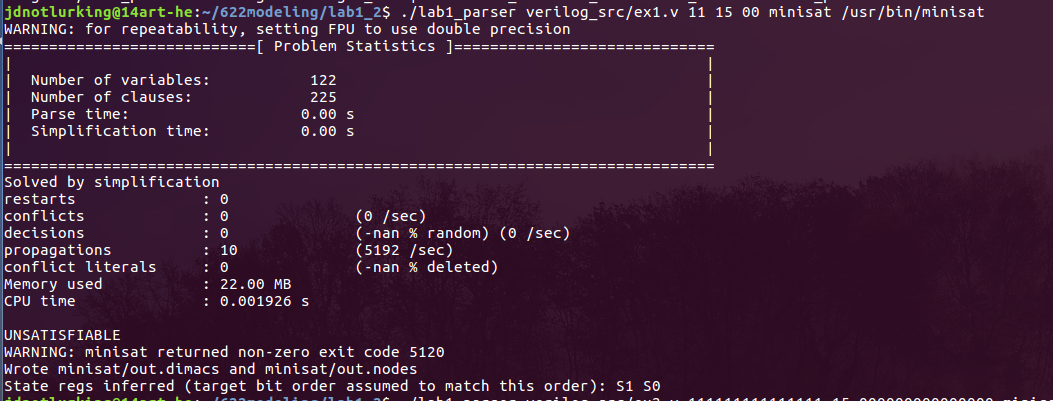
\includegraphics[width=0.9\textwidth]{minisat_ex1.png}
\caption{SAT solver result for \texttt{ex1} (UNSAT).}
\end{figure}

\textbf{ex2}

Target state consisting of all ones was not reachable within the 15-step bound.

\begin{figure}[H]
\centering
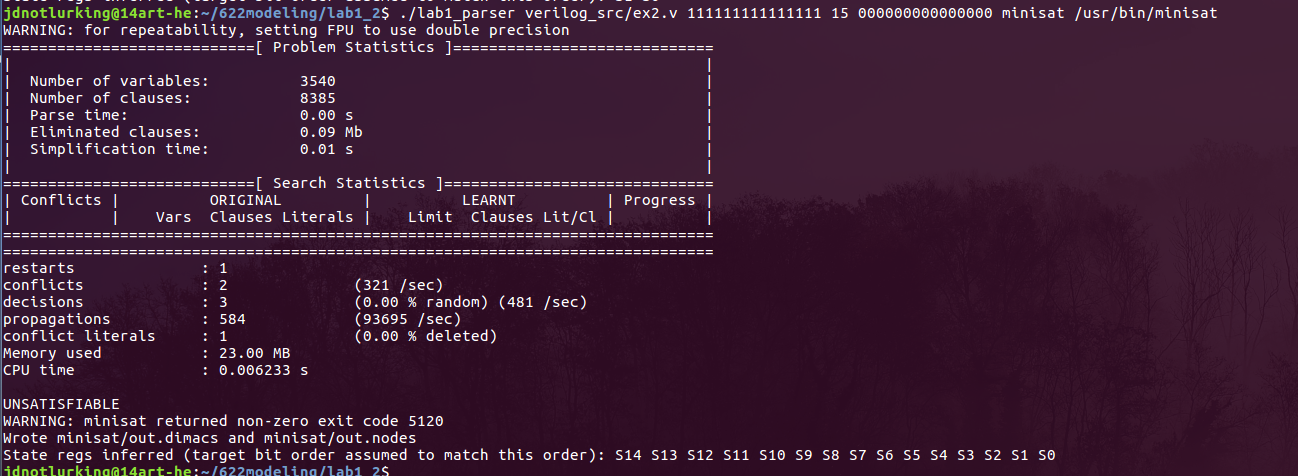
\includegraphics[width=0.9\textwidth]{minisat_ex2.png}
\caption{SAT solver result for \texttt{ex2} (UNSAT).}
\end{figure}

\textbf{ex3}

The solver returned \textbf{SAT}, indicating that the target state is reachable within the unrolling bound.

\begin{figure}[H]
\centering
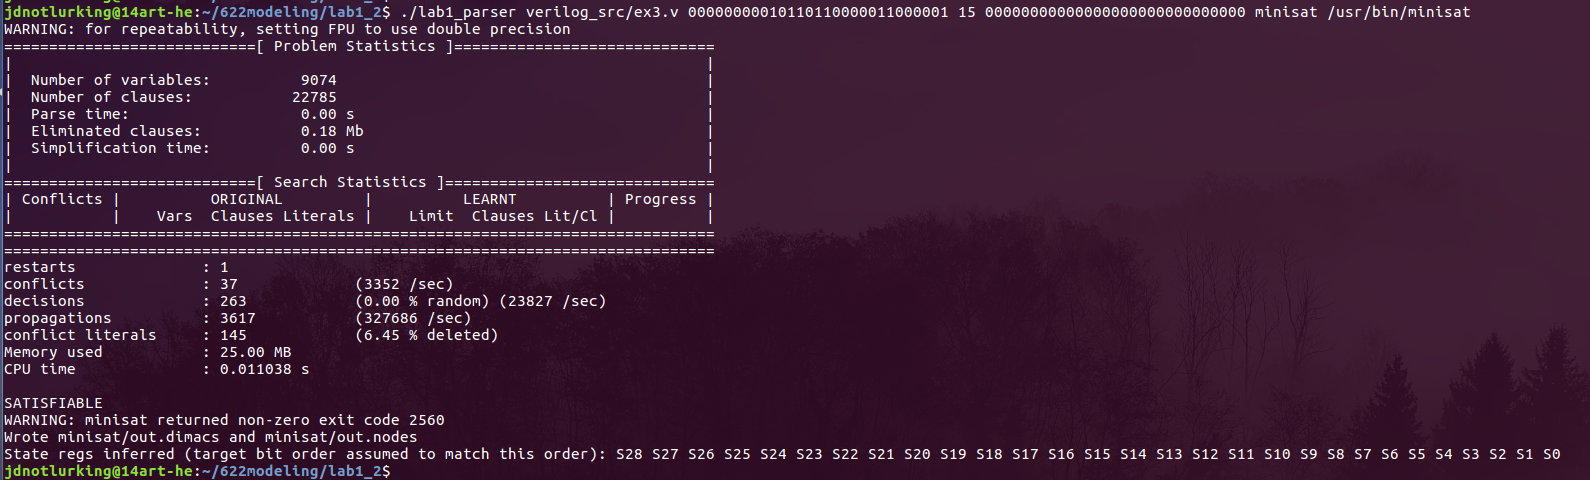
\includegraphics[width=0.9\textwidth]{minisat_ex3.png}
\caption{SAT solver result for \texttt{ex3} (SAT).}
\end{figure}

\textbf{ex4}

The solver returned \textbf{UNSAT}, indicating the target state is not reachable within 15 transitions.

\begin{figure}[H]
\centering
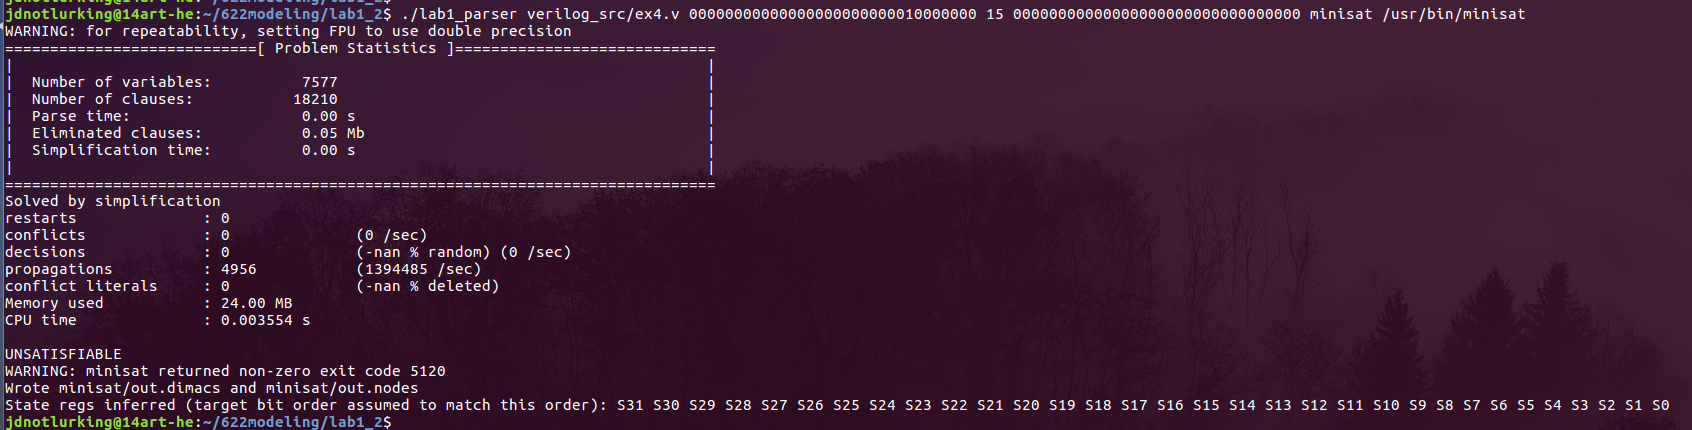
\includegraphics[width=0.9\textwidth]{minisat_ex4.png}
\caption{SAT solver result for \texttt{ex4} (UNSAT).}
\end{figure}

\textbf{ex5}

The solver returned \textbf{UNSAT}, meaning the specified target state cannot be reached within the bound.

\begin{figure}[H]
\centering
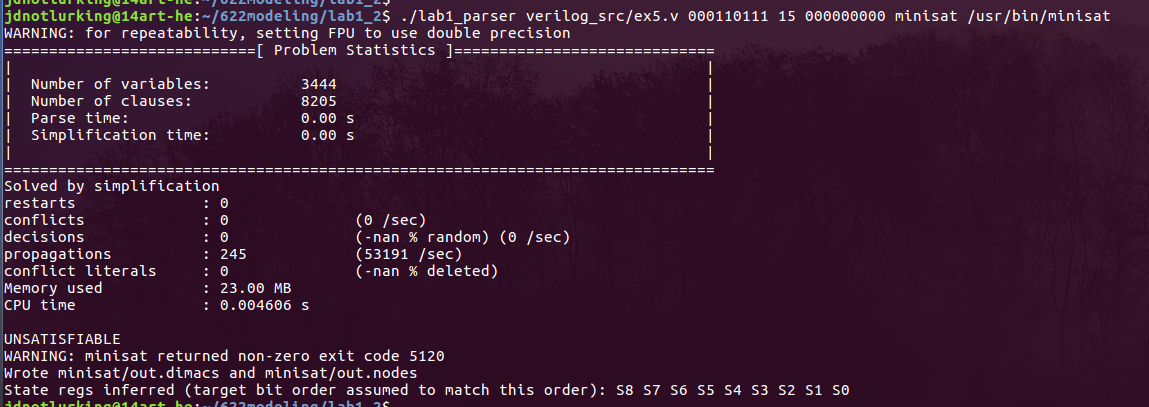
\includegraphics[width=0.9\textwidth]{minisat_ex5.png}
\caption{SAT solver result for \texttt{ex5} (UNSAT).}
\end{figure}

\textbf{stoplight1}

The solver returned \textbf{SAT}, confirming that the target state \texttt{0100} is reachable within the 15-step bound.

\begin{figure}[H]
\centering
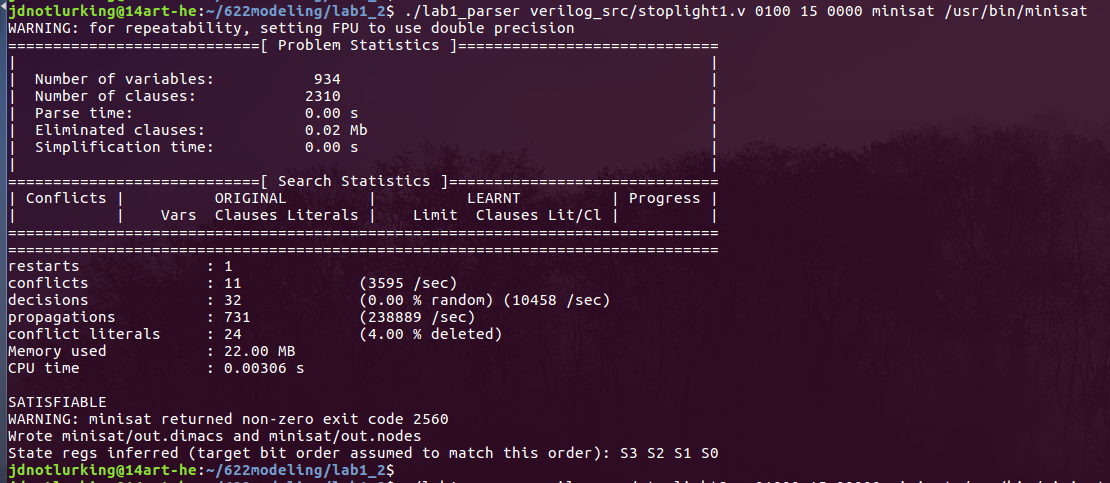
\includegraphics[width=0.9\textwidth]{minisat_stoplight1.png}
\caption{SAT solver result for \texttt{stoplight1} (SAT).}
\end{figure}

\textbf{stoplight2}

The solver returned \textbf{SAT}, confirming that the target state \texttt{01000} is reachable.

\begin{figure}[H]
\centering
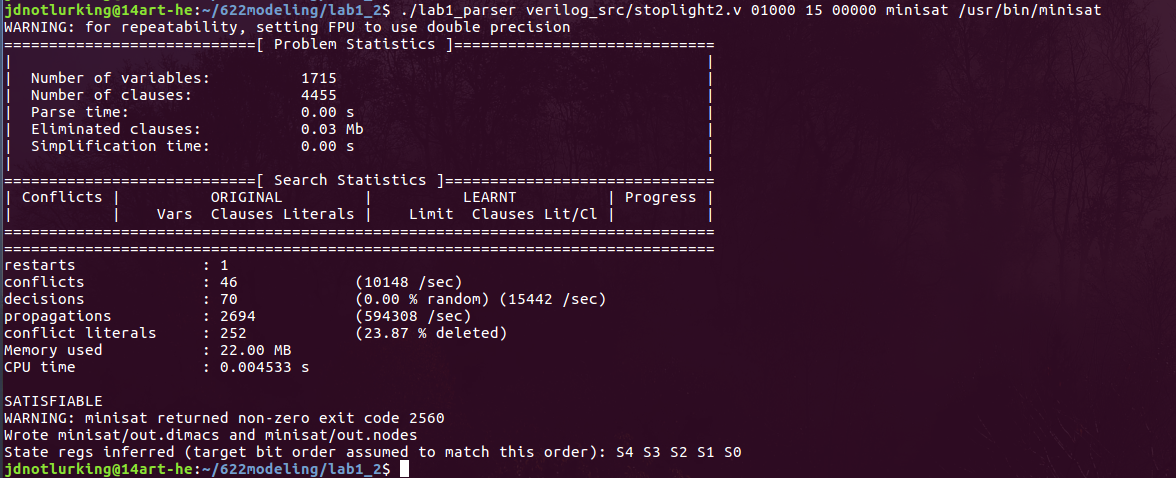
\includegraphics[width=0.9\textwidth]{minisat_stoplight2.png}
\caption{SAT solver result for \texttt{stoplight2} (SAT).}
\end{figure}

% ------------------------------------------------------------
% B.3
% ------------------------------------------------------------
\subsection*{B.3: stoplight1 Reachable on i-th Transition (1–32)}

To determine for which transition index $i$ the target state becomes reachable, we invoked the SAT-based reachability tool repeatedly while varying the unrolling depth from $i=1$ to $i=32$. For each value of $i$, the transition relation was unrolled $i$ times and the solver was asked whether the target state \texttt{0100} could be reached from the initial state \texttt{0000}.

The SAT solver reported \textbf{UNSAT} for values $i < 12, i \neq 4$ and has \textbf{SAT} solutions for values $i \geq 12$ and $i=4$.


\textbf{Reachable indices:}

\[
i = \{4, 12, 13 \dots, 31, 32\}
\]

This means that although the shortest path in the state graph may require fewer transitions, the bounded model checking formulation detects reachability starting at $i=12$.

---

% ------------------------------------------------------------
% B.4
% ------------------------------------------------------------
\subsection*{B.4: stoplight2 Comparison with Random Simulation}

Using the same symbolic reachability procedure, the solver was invoked for increasing transition depths $i$ from $1$ to $32$ for the circuit \texttt{stoplight2.v}. The target state considered was \texttt{01000}.

The solver returned \textbf{UNSAT} for all values $i < 14$ and \textbf{SAT} for all values $i \geq 14$.

\textbf{Reachable indices:}

\[
i = \{14, 15, 16, \dots, 31, 32\}
\]

\textbf{Comparison with A.4 (Random Simulation)}

In Section A.4, random simulation reached the same target state after 1357 clock cycles. The symbolic SAT-based analysis here determines the earliest transition depth at which the state becomes reachable, independent of any particular input sequence.

Thus, symbolic reachability analysis provides a deterministic bound on reachability, while random simulation may take significantly longer to encounter the required sequence of inputs.


% ------------------------------------------------------------
% B.5
% ------------------------------------------------------------
\subsection*{B.5: States Reachable on the 17th Transition (stoplight2)}

To determine the set of states reachable exactly at transition $k=17$, we computed the set $\delta^{17}(S_0)$ using SAT-based reachability analysis.

\textbf{Approach}

\begin{itemize}
\item The transition relation was unrolled for $k = 17$ steps starting from the fixed initial state.
\item For each candidate state $s$, unit clauses were added constraining the state variables at time step 17 to equal $s$.
\item The SAT solver was invoked to determine whether a satisfying assignment exists.
\item If the solver returned SAT, this indicates that there exists an input sequence of length 17 that drives the FSM from the initial state to $s$.
\item This procedure was repeated for all $2^5 = 32$ possible states of the FSM.
\end{itemize}

Using this method, the following \textbf{19 states} were found to be reachable at the 17th transition:

\[
\begin{aligned}
\{00000, 00001, 00010, 00011, 00100, 00101, 00110, 00111, 01000, 01001,\\
10000, 10001, 10010, 10011, 10100, 10101, 10110, 10111, 11000\}
\end{aligned}
\]
These states represent all configurations for which a valid sequence of 17 inputs exists that leads from the initial state to the specified state.

%%%%%%%%%%%%%%%%%%%%%%%%%%%%%%%%%%%%%%%%%%%%%%%%%%
\section{Part C: Counting Reachable States (ECE 622)}

\subsection*{C.1: Reachable States in ex5 and ex1}



% In body:
\begin{table}[H]
\centering
\caption{Part C (ex5): Number of reachable states at transition $i$}
\label{tab:ex5_partc_reach}
\begin{tabular}{c c}
\toprule
$i$ & SAT count \\
\midrule
1  & 8/512  \\
2  & 14/512 \\
3  & 18/512 \\
4  & 22/512 \\
5  & 26/512 \\
6  & 28/512 \\
7  & 28/512 \\
8  & 28/512 \\
9  & 28/512 \\
10 & 28/512 \\
11 & 28/512 \\
12 & 28/512 \\
13 & 28/512 \\
14 & 28/512 \\
15 & 28/512 \\
16 & 28/512 \\
17 & 28/512 \\
18 & 28/512 \\
19 & 28/512 \\
20 & 28/512 \\
\bottomrule
\end{tabular}
\end{table}

\begin{table}[H]
\centering
\caption{Part C (ex1): Reachable target states at transition $i$ (MiniSat SAT results)}
\label{tab:ex1_partc_reach}
\begin{tabular}{c c}
% \begin{tabularx}{\linewidth}{@{}r c X@{}}
\toprule
$i$ & SAT count \\
\midrule
% 0  & 1/4 & -- \\
1  & 1/4 \\
2  & 1/4 \\
3  & 1/4\\
4  & 1/4 \\
5  & 1/4 \\
6  & 1/4 \\
7  & 1/4 \\
8  & 1/4 \\
9  & 1/4 \\
10 & 1/4 \\
11 & 1/4 \\
12 & 1/4 \\
13 & 1/4 \\
14 & 1/4 \\
15 & 1/4 \\
16 & 1/4 \\
17 & 1/4 \\
18 & 1/4 \\
19 & 1/4 \\
20 & 1/4 \\
% ... continue up to your max i for ex1 (maybe 20 or 32 depending on the prompt)
\bottomrule
\end{tabular}
\end{table}


\subsection*{C.2: Approach Description}

Our approach to counting reachable states:

\begin{itemize}
\item Iteratively unrolled transition relation.
\item Used SAT solver to check existence.
\item Added blocking clauses to enumerate unique states.
\item Maintained cumulative set of reachable states.
\end{itemize}

Code submitted separately on canvas. (\texttt{minisat\_reach\_table.cpp} and \texttt{partc\_hashmap.sh})

%%%%%%%%%%%%%%%%%%%%%%%%%%%%%%%%%%%%%%%%%%%%%%%%%%

\section*{Use of Tools}

We used the following tools in completing this lab:

\begin{itemize}
\item MiniSAT / PicoSAT on Ubuntu 14.
\item AMD Vivado 2025.1 on Windows 10.
\item C++ for CNF generation
\item TikZ for graph visualization
\item ChatGPT for assistance in structuring Lab report.
\end{itemize}

AI prompts and descriptions are included in the appendix.

%%%%%%%%%%%%%%%%%%%%%%%%%%%%%%%%%%%%%%%%%%%%%%%%%%

%%%%%%%%%%%%%%%%%%%%%%%%%%%%%%%%%%%%%%%%%%%%%%%%%%
%%%%%%%%%%%%%%%%%%%%%%%%%%%%%%%%%%%%%%%%%%%%%%%%%%
\appendix
\section*{Appendix}
\addcontentsline{toc}{section}{Appendix}

%%%%%%%%%%%%%%%%%%%%%%%%%%%%%%%%%%%%%%%%%%%%%%%%%%
\subsection*{A. Testbench Used for Random Simulation (A.4)}

\begin{figure}[H]
\centering
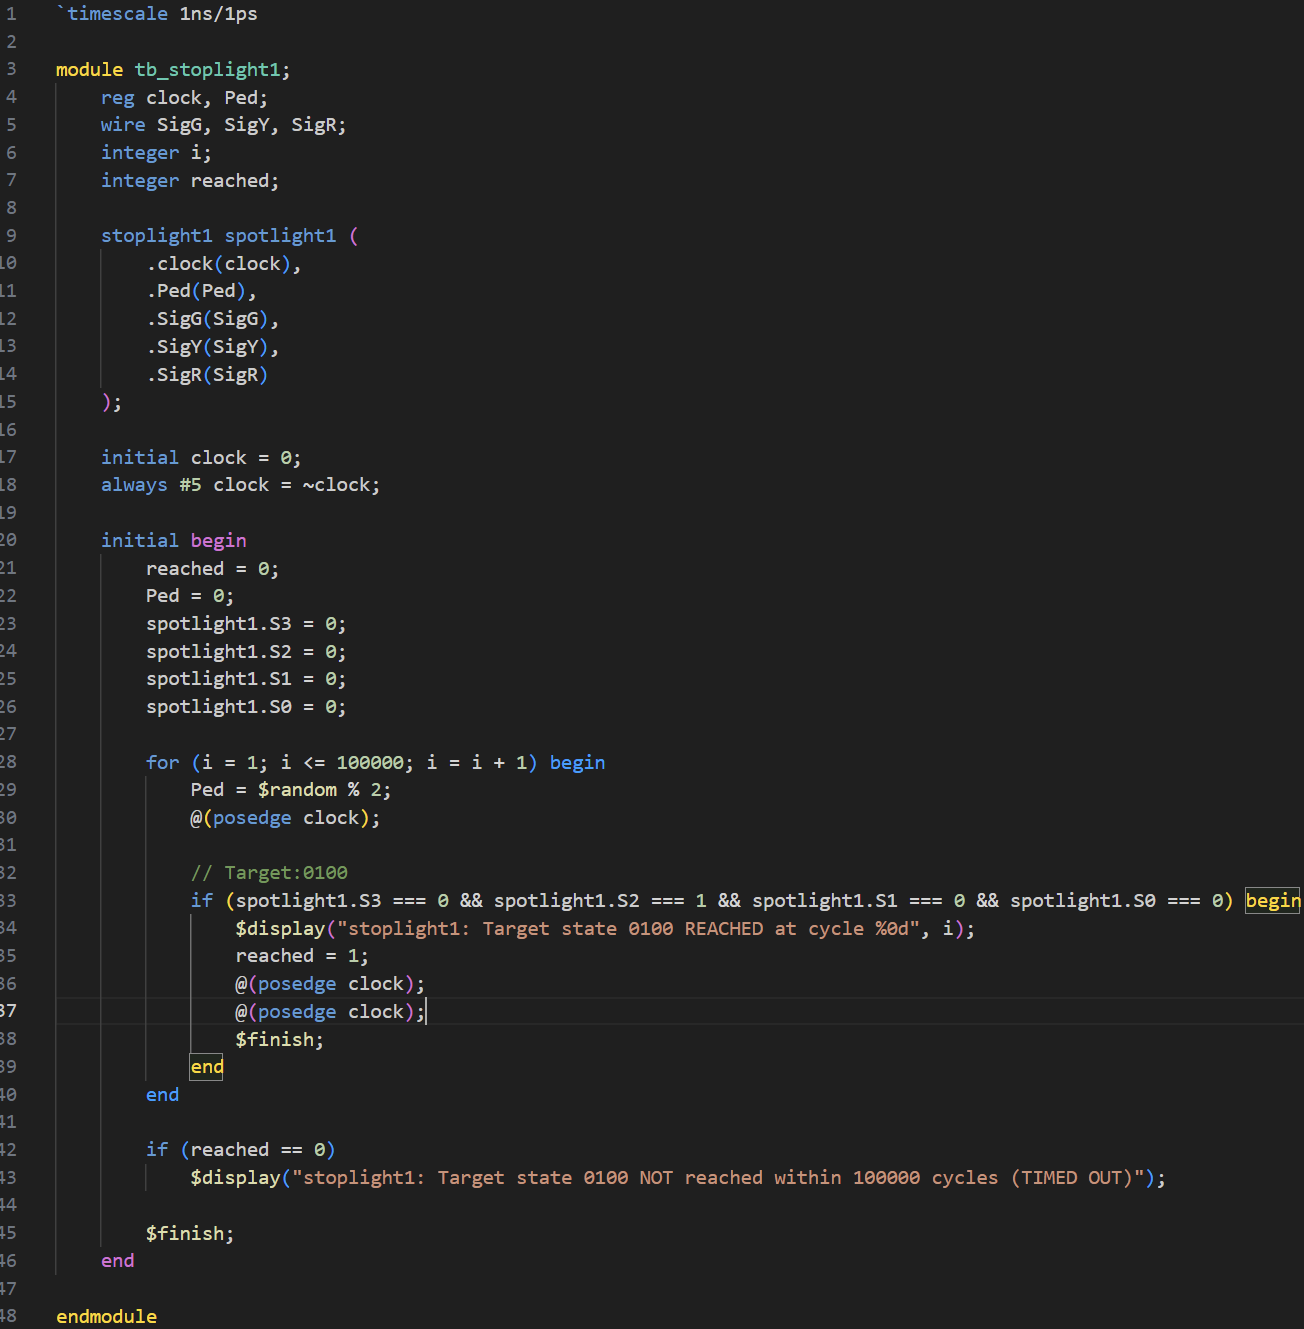
\includegraphics[width=0.9\textwidth]{testbench.png}
\caption{Verilog testbench used for random execution experiments in Section A.4.}
\end{figure}

The testbench initializes the FSM to its starting state and applies randomized values to the input signal \texttt{Ped} at each clock cycle. The simulation terminates when the target state is reached or after a fixed number of cycles.


\begin{figure}[H]
\centering
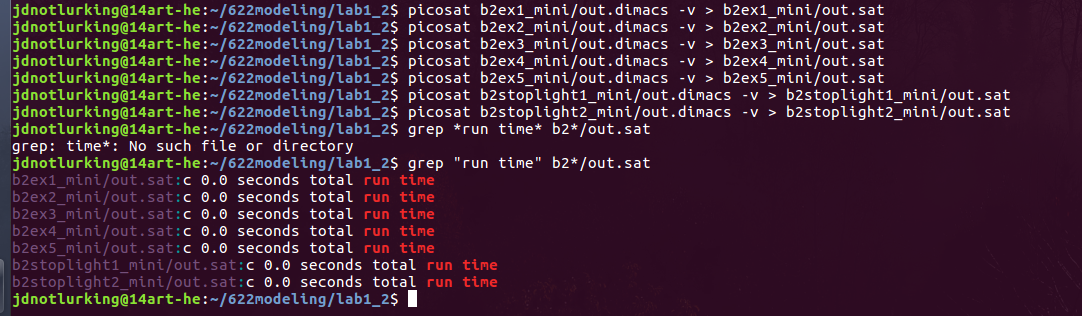
\includegraphics[width=0.9\textwidth]{picosattime.png}
\caption{Picosat solver run time measurements}
\end{figure}
%%%%%%%%%%%%%%%%%%%%%%%%%%%%%%%%%%%%%%%%%%%%%%%%%%
\subsection*{B. Prompts Used for Tool Assistance}

As required by the lab instructions, we document the prompts used when employing AI-based tools to assist with diagram generation, formatting, and documentation. AI assistance was used only as a productivity aid for generating templates or converting information into LaTeX format; all logic analysis, reachability reasoning, and correctness verification were performed manually.

\subsubsection*{B.1 Prompt for Generating the ex1 FSM Graph}

% \textbf{Prompt used:}
Prompt Used:
\begin{verbatim}
Generate a TikZ template for a 4-state FSM graph with labeled transitions 
that I can adapt for reachability analysis in Verilog.
\end{verbatim}

% \textbf{Purpose:}
Purpose:
This prompt was used to generate an initial TikZ template for a small FSM diagram. The final diagram in the report therefore reflects the manually derived state transition relation.

%%%%%%%%%%%%%%%%%%%%%%%%%%%%%%%%%%%%%%%%%%%%%%%%%%
\subsubsection*{B.2 Prompt for Generating the stoplight1 FSM Layout}

% \textbf{Prompt used:}
Prompt Used:

\begin{verbatim}
Generate a TikZ diagram for a 16-state FSM arranged in a circular layout.
Transitions should be labeled with Ped input values, with white
background labels to keep them readable. Allow color-coded states
according to a reference table and highlight a specific path of
transitions in red.
\end{verbatim}

% \textbf{Purpose:}
Purpose:

This prompt was used to obtain a structural template for visualizing a larger FSM containing 16 possible states.


%%%%%%%%%%%%%%%%%%%%%%%%%%%%%%%%%%%%%%%%%%%%%%%%%%
\subsubsection*{B.3 Prompt for Converting Screenshots into LaTeX Tables}

% \textbf{Prompt used:}
Prompt Used:
\begin{verbatim}
Convert the numerical data shown in the attached screenshot into a
properly formatted LaTeX table suitable for inclusion in an academic report.
\end{verbatim}

% \textbf{Purpose:}
Purpose:
ChatGPT is very quick at processing screenshot (of logs / other documents) and converting them to report-friendly text. Hence we used prompts to convert tabulated experimental results from screenshots into LaTeX table format. The resulting tables were then reviewed and manually verified to ensure consistency with the reachability experiments. This assisted in producing Tables \ref{tab:a3_ex1} and \ref{tab:a3_stoplight1} in Section A.3.

%%%%%%%%%%%%%%%%%%%%%%%%%%%%%%%%%%%%%%%%%%%%%%%%%%
\subsection*{C. Additional Notes}

\begin{itemize}
\item GitHub repository containing all source code and scripts used for this lab:

\url{https://github.com/JDKhare/UMass_ECE622_Labs/tree/main/lab1}
\end{itemize}

\end{document}




% \section*{Overview}

% All experiments were performed on Ubuntu 16.04 using MiniSAT and PicoSAT.

% % =================================================
% % Part A
% % =================================================

% \section{Part A: Reachability by Graph Traversal}

% We determined reachability using explicit checks: pen and paper for drawing the graph, and AMD Vivado for random execution. 
% % -------------------------------------------------
% % A.1
% % -------------------------------------------------
% \subsection*{A.1: State transition graph for ex1 and stoplight1}

% \begin{figure}[h]
% \centering
% \begin{tikzpicture}[->, >=stealth, node distance=3cm, on grid, auto]

% \node[state] (S0) {$S_0$};
% \node[state] (S1) [right=of S0] {$S_1$};
% \node[state] (S2) [below=of S0] {$S_2$};

% \path
% (S0) edge node {a} (S1)
% (S1) edge node {b} (S2)
% (S2) edge[bend right] node {c} (S0);

% \end{tikzpicture}
% \caption{State Transition Graph for ex1.v}
% \end{figure}

% Annotated graph for ex1 and stoplight1. (Generated using TikZ!)

% % A.2

% % A.3
% % A.4
% % A.5


% While this section A was a good exercise to understand step by step how we can brute force reachability, it sure was tedious and the need for more formal methods is apparent. 


% % =================================================
% % Part B
% % =================================================
% The given problem was first translated into Conjunctive Normal Form (CNF).
% Each Boolean variable was assigned an integer index according to the mapping file
% (\texttt{out.nodes}).

% The DIMACS file follows the structure:

% \begin{verbatim}
% c comment line
% p cnf <num_variables> <num_clauses>
% <clause 1> 0
% <clause 2> 0
% ...
% \end{verbatim}

% \subsection*{RESULT 1.1: Example DIMACS File}

% \begin{verbatim}
% c Example SAT instance
% p cnf 3 3
% 1 0
% 2 0
% -1 3 0
% \end{verbatim}

% Where:
% \begin{itemize}
%     \item Variable 1 represents node A
%     \item Variable 2 represents node B
%     \item Variable 3 represents node C
% \end{itemize}
% \section{Step 2: Running MiniSAT and PicoSAT}

% \subsection*{RESULT 2.1: Running MiniSAT}

% Command used:

% \begin{verbatim}
% minisat example.cnf output.txt
% \end{verbatim}

% Output:

% \begin{verbatim}
% SAT
% 1 2 3 0
% \end{verbatim}

% Interpretation:
% \begin{itemize}
%     \item Variable 1 = TRUE
%     \item Variable 2 = TRUE
%     \item Variable 3 = TRUE
% \end{itemize}

% \subsection*{RESULT 2.2: Running PicoSAT}

% Command used:

% \begin{verbatim}
% picosat example.cnf
% \end{verbatim}

% Output:

% \begin{verbatim}
% s SATISFIABLE
% v 1 2 3 0
% \end{verbatim}

% Both solvers returned consistent results.

% % =================================================
% % STEP 3: UNSAT CASE
% % =================================================

% \section{Step 3: UNSAT Example}

% To validate correctness, an UNSAT case was created:

% \begin{verbatim}
% p cnf 1 2
% 1 0
% -1 0
% \end{verbatim}

% Both solvers returned:

% \begin{verbatim}
% UNSAT
% \end{verbatim}

% This confirms proper CNF formatting and solver setup.

% % =================================================
% % STEP 4: INTERPRETING SOLVER OUTPUT
% % =================================================

% \section{Step 4: Mapping Solver Output to Nodes}

% The solver output assigns truth values to integer-indexed variables.
% Using the mapping file:

% \[
% x_i = 1 \Rightarrow \text{Node } i = TRUE
% \]
% \[
% x_i = -1 \Rightarrow \text{Node } i = FALSE
% \]

% This mapping allows verification of reachability or logical property satisfaction.

% % =================================================
% % STEP 5: OPTIONAL GRAPH VISUALIZATION
% % =================================================

% \section{Step 5: Graph Visualization (Optional)}

% To visualize implication or reachability graphs, Graphviz was used.

% Example \texttt{.dot} file:

% \begin{verbatim}
% digraph G {
%     A -> B;
%     B -> C;
% }
% \end{verbatim}

% Generated using:

% \begin{verbatim}
% dot -Tpdf graph.dot -o graph.pdf
% \end{verbatim}

% This visualization assists in debugging CNF encodings.

% % =================================================
% % CONCLUSION
% % =================================================

% \section*{Conclusion}

% In this lab, CNF encodings were generated and validated using MiniSAT and PicoSAT.
% Both SAT and UNSAT instances were successfully verified.
% The exercise demonstrates how logical reasoning problems can be reduced to SAT
% and solved efficiently using modern solvers.

% This forms the foundation for SAT-based reachability, equivalence checking,
% and formal verification techniques used in modern CAD tools.

% \end{document}
